\documentclass{standalone}

\usepackage{textcomp}
\usepackage{amsmath,amsfonts,amssymb,amstext}
\usepackage{graphicx,color}
\usepackage[hang]{caption}
% TIKZ
\usepackage{tikz}
\usetikzlibrary{arrows,backgrounds,positioning,decorations,decorations.pathreplacing,shapes}
\newcommand{\data}[5]{\draw [#1] (#3,#2) -- ++(#4-#3,0) node[midway,above] {\small #5} ;}
% Include Tikz images
\newcommand{\inputTikz}[2][1]{%
  \centering
  \scalebox{#1}{
   \input{#2.tikz}%
}}
\input{commands.tex}

\begin{document}

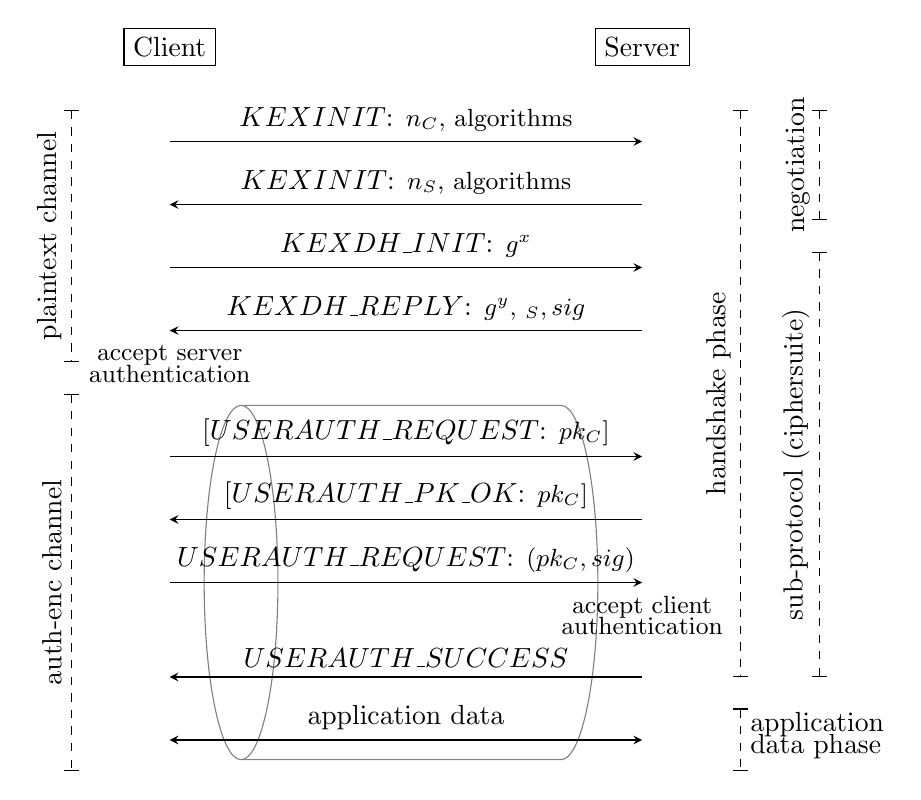
\begin{tikzpicture}[>=stealth,yscale=-0.8]
\newcommand{\xInit}{0}
\newcommand{\xResp}{6}
\newcommand{\arrWidth}{6}
\newcommand{\leftVert}{-1.25}
\newcommand{\rightVert}{7.25}

\draw (\xInit,-0.5) node[rectangle,draw] {Client};
\draw (\xResp,-0.5) node[rectangle,draw] {Server};

% negotiation
\draw[->] (\xInit,1) -- node[above] {$\msg{KEXINIT}$: \small $n_C$, algorithms} +(\arrWidth,0);
\draw[<-] (\xInit,2) -- node[above] {$\msg{KEXINIT}$: \small $n_S$, algorithms} +(\arrWidth,0);
% DH
\draw[->] (\xInit,3) -- node[above] {$\msg{KEXDH\_INIT}$: \small $g^x$} +(\arrWidth,0);
\draw[<-] (\xInit,4) -- node[above] {$\msg{KEXDH\_REPLY}$: \small $g^y$, $\pk_{S}, sig$} +(\arrWidth,0);
\draw (\xInit,4.4) node {\small accept server};
\draw (\xInit,4.4) node[below] {\small authentication};
% auth-enc channel
\node[draw,cylinder,rotate=180,shape aspect=4,minimum height=5cm,minimum width=4.5cm,gray] at (3.25,8) {};
\draw[->] (\xInit,6) -- node[above] {$\msg{[USERAUTH\_REQUEST}$: \small $pk_{C}]$} +(\arrWidth,0);
\draw[<-] (\xInit,7) -- node[above] {$\msg{[USERAUTH\_PK\_OK}$: \small $pk_{C}]$} +(\arrWidth,0);
\draw[->] (\xInit,8) -- node[above] {$\msg{USERAUTH\_REQUEST}$: \small $(pk_{C}, sig)$} +(\arrWidth,0);
\draw (\xResp,8.4) node {\small accept client};
\draw (\xResp,8.4) node[below] {\small authentication};
\draw[<-] (\xInit,9.5) -- node[above] {$\msg{USERAUTH\_SUCCESS}$ } +(\arrWidth,0);
\draw[<->] (\xInit,10.5) -- node[above] {application data} +(\arrWidth,0);

% channels
\draw[|-|,dashed] (\leftVert,0.5) -- node[above,rotate=90] {plaintext channel} +(0,4);
\draw[|-|,dashed] (\leftVert,5) -- node[above,rotate=90] {auth-enc channel} +(0,6);

% phases
\draw[|-|,dashed] (\rightVert,0.5) -- node[above,rotate=90] {handshake phase} +(0,9);
\draw[|-|,dashed] (\rightVert,10) -- +(0,1);
\draw (\rightVert,10.25) node[right] {application};
\draw (\rightVert,10.25) node[below right] {data phase};
\draw[|-|,dashed] (\rightVert+1,0.5) -- node[above,rotate=90] {negotiation} +(0,1.75);
\draw[|-|,dashed] (\rightVert+1,2.75) -- node[above,rotate=90] {sub-protocol (ciphersuite)} +(0,6.75);

\end{tikzpicture}

\end{document}